\documentclass[border=8pt]{standalone}
\usepackage{fontspec}
\setmainfont{TeX Gyre Heros}[Ligatures=TeXOff]
\XeTeXgenerateactualtext=1
\setsansfont{TeX Gyre Heros}
\usepackage{tikz}
\usetikzlibrary{arrows.meta,positioning,shapes.geometric,shapes.misc,shapes.symbols,fit,backgrounds,calc,chains}
\definecolor{ink}{HTML}{111827}
\definecolor{band}{HTML}{F3F4F6}
\definecolor{band2}{HTML}{E5E7EB}
\definecolor{accent}{HTML}{1D4ED8}
\definecolor{accentlight}{HTML}{DBEAFE}
\definecolor{warn}{HTML}{B91C1C}
\definecolor{warnlight}{HTML}{FEE2E2}
\definecolor{ok}{HTML}{047857}
\definecolor{oklight}{HTML}{D1FAE5}
\tikzset{
  >={Stealth[length=2.6mm]},
  box/.style={draw=ink, line width=0.6pt, rounded corners=9pt, fill=white, align=center,
              inner sep=4pt, font=\small},
  pill/.style={box, rounded corners=13pt},
  key/.style={box, fill=accentlight, draw=accent, line width=0.9pt},
  soft/.style={box, fill=band},
  dec/.style={draw=ink, line width=0.6pt, diamond, aspect=2.2, align=center, inner sep=1.5pt,
              font=\footnotesize, fill=white},
  arr/.style={->, draw=ink, line width=0.6pt},
  darr/.style={->, draw=ink, line width=0.6pt, dashed},
  lbl/.style={font=\footnotesize, fill=white, inner sep=1.5pt},
  layer/.style={draw=band2, fill=band, rounded corners=6pt},
  title/.style={font=\bfseries\small, align=left, anchor=west},
}
\begin{document}
\sffamily\hyphenpenalty=10000\exhyphenpenalty=10000

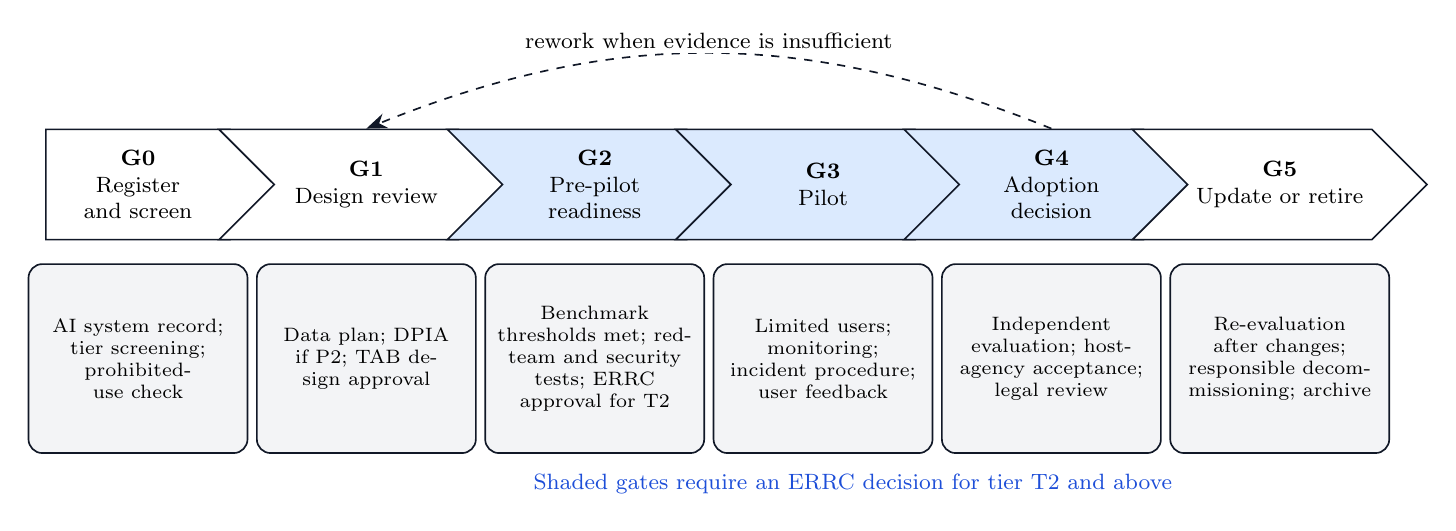
\begin{tikzpicture}
\tikzset{g/.style={draw=ink, line width=0.6pt, fill=white, signal, signal to=east, signal from=west,
                   minimum height=14mm, minimum width=28mm, align=center, font=\footnotesize, text width=22mm, inner sep=2pt},
         ev/.style={box, font=\scriptsize, text width=25mm, minimum height=24mm, anchor=north, fill=band, rounded corners=5pt}}
\node[g, signal from=nowhere] (g0) at (0,0) {\textbf{G0}\\Register and screen};
\node[g] (g1) at (29mm,0) {\textbf{G1}\\Design review};
\node[g, fill=accentlight] (g2) at (58mm,0) {\textbf{G2}\\Pre-pilot readiness};
\node[g, fill=accentlight] (g3) at (87mm,0) {\textbf{G3}\\Pilot};
\node[g, fill=accentlight] (g4) at (116mm,0) {\textbf{G4}\\Adoption decision};
\node[g] (g5) at (145mm,0) {\textbf{G5}\\Update or retire};
\node[ev] at (0,-10mm) {AI system record; tier screening; prohibited-use check};
\node[ev] at (29mm,-10mm) {Data plan; DPIA if P2; TAB design approval};
\node[ev] at (58mm,-10mm) {Benchmark thresholds met; red-team and security tests; ERRC approval for T2};
\node[ev] at (87mm,-10mm) {Limited users; monitoring; incident procedure; user feedback};
\node[ev] at (116mm,-10mm) {Independent evaluation; host-agency acceptance; legal review};
\node[ev] at (145mm,-10mm) {Re-evaluation after changes; responsible decommissioning; archive};
\draw[darr] (g4.north) to[bend right=22] node[lbl, above]{rework when evidence is insufficient} (g1.north);
\node[font=\footnotesize, anchor=west, text=accent] at (49mm,-38mm) {Shaded gates require an ERRC decision for tier T2 and above};
\end{tikzpicture}
\end{document}
